\documentclass[12pt,a4paper]{report}
\usepackage[utf8]{vietnam}
\usepackage[utf8]{inputenc}
\usepackage{tabto}
\usepackage{amsmath}
\usepackage{amsfonts}
\usepackage{tikz}
\usepackage{amssymb}
\usepackage{graphicx}
\usepackage[left=2cm,right=2cm,top=2cm,bottom=2cm]{geometry}
\usepackage{graphicx}
\graphicspath{ {./images/} }

\author{Trần Đức Mạnh}
\title{Deep Learning}
\begin{document}
\tableofcontents

\chapter{Practical Aspects of Deep Learning}
	\section{Deep $L$ - Layer Neural Network}
		\subsection{Notation}
		\subsection{Chiều của các Ma trận}
	\section{Setting up your Machine Learning Application}
		\subsection{Train/Dev/Test sets}
		\subsection{Bias/Variance}
		\subsection{Basic Recipe for Machine Learning (“Công thức cơ bản” để xử lý High Bias với High Variance)}
	\section{Regularizing your Neural Network}
		\subsection{Regularization}
		\subsection{Cách Regularization giảm Overfitting}
		\subsection{Dropout Regularization}
		\subsection{Một số cách để giảm Overfitting khác}
	\section{Setting up your Optimization Problem}
\chapter{Optimization Algorithms}
	\section{Mini-batch Gradient Descent}
	\section{Exponentially weighted averages}
		\begin{itemize}
			\item Ý tưởnga: Khiến cho phân bố của các giá trị trở nên "smooth" hơn
			\item Tại sao cần đến: Khiến cho thuật toán chạy nhanh hơn, train model nhanh hơn
			\item Hình ảnh trực quan \\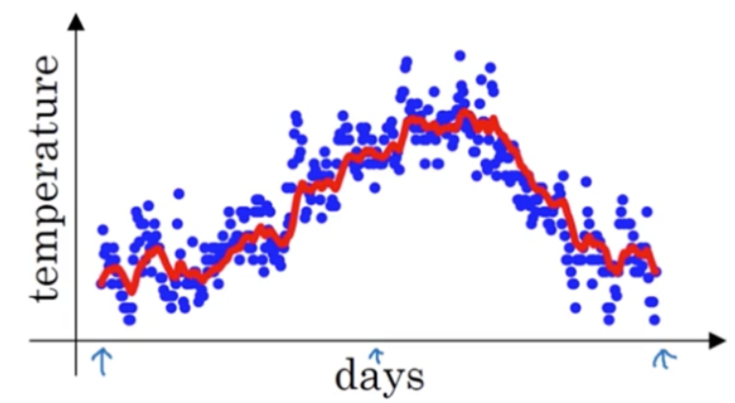
\includegraphics[scale=0.5]{1}
			\item Công thức:
				\[ v_t = \beta v_{t-1} + (1 - \beta)\theta_t \]
				\begin{itemize}
					\item $ \beta $ là 1 hyperparameter
					\item $ \beta $ tăng thì đồ thị càng "smooth", giảm thì độ thị càng "noisy"
					\item $ \theta_t $ là giá tương ứng tại t
				\end{itemize}
			\item Implementation: \\
				$v_\theta = 0$ \\
				repeat \{ \\
				\tabto{0.5cm} get next $\theta_t$ \\ 
				\tabto{0.5cm} $ v_\theta := \beta v_\theta + (1 - \beta) \theta_t $ \\
				\}	
			\item Bias correction:
				\begin{itemize}
					\item Vấn đề: đồ thị bị thấp hơn so với bao đầu \\
					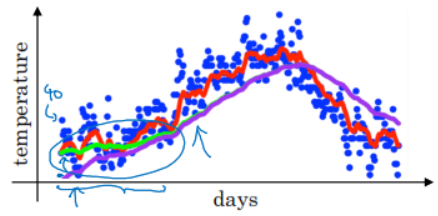
\includegraphics[scale=0.8]{2} \\
 					\tabto{0.5cm} Đường màu tím có điểm bắt đầu rất thấp do khởi tạo $ v_\theta = 0 $
 					\item Khắc phục: chia $ v_\theta $ cho $ 1 - \beta^t $
				\end{itemize}
		\end{itemize}
	\section{Gradient Descent with Momentum}
		\begin{itemize}
			\item Ý tưởng: Thay vì áp dụng trực tiếp Gradient Descent, ta áp dụng Exponential weighted averages lên $d\omega$ và $db$ để khiến thuật toán Gradient Descent chạy nhanh hơn.\\
				\tabto{0.5cm} Hình ảnh minh hoạ: \\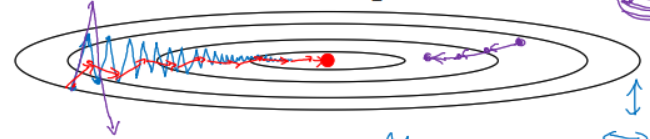
\includegraphics[scale=0.6]{3} \\
				\tabto{0.5cm} Biến đường màu xanh thành đường màu đỏ
			\item Implemetation: \\
				On iteration $t$:
				\tabto{0.5cm} Compute $ d\omega, db $ on current mini-batch \\
				\tabto{0.5cm} $ V_{d\omega} = \beta V_{d\omega} + (1 - \beta) d\omega $ \\
				\tabto{0.5cm} $ V_{db} = \beta V_{db} + (1 - \beta) db $ \\
				\tabto{0.5cm} $ \omega := \omega - \alpha V_{d\omega}, b := b - \alpha V_{db} $ \\
		\end{itemize}
	\section{RMSprop}
		\begin{itemize}
			\item Tên đầy đủ: Root Mean Square prop
			\item Ý tưởng: tương tự như \textbf{Gradient Descent with Momentum}
			\item Implementation: \\
				On iteration $t$:
				\tabto{0.5cm} Compute $d\omega, db$ on current mini-batch \\
				\tabto{0.5cm} $ S_{d\omega} = \beta S_{d\omega} + (1 - \beta) d_\omega^2 $ (square element-wise)\\
				\tabto{0.5cm} $ S_{db} = \beta S_{db} + (1 - \beta) d_b^2 $\\
				\tabto{0.5cm} $ \omega := \omega - \alpha \frac{d\omega}{\sqrt{S_{d\omega}}}, b := b - \alpha \frac{db}{\sqrt{S_{db}}} $\\
		\end{itemize}
	\section{Adam Optimization Algorithm}
		\begin{itemize}
			\item Tên đầy đủ: Adaptive Moment Estimation
			\item ý tưởng: Kết hợp \textbf{Gradient Descent with Momentum} và \textbf{RMSprop}
			\item Implementation: \\
				$ V_{d\omega} = 0, S_{d\omega} = 0 $ \\
				$ V_{db} = 0, S_{db} = 0 $ \\
				On iterate $t$: \\
				\tabto{0.5cm} Compute $ d\omega, db $ using current mini-batch\\
				\tabto{0.5cm} $ V_{d\omega} = \beta_1 V_{d\omega} + (1 - \beta_1) d\omega, V_{db} = \beta_1 V_{db} + (1 - \beta_1) db $ (\textit{moment} with hyperpara $ \beta_1 $)\\
				\tabto{0.5cm} $ S_{d\omega} = \beta_2 S_{d\omega} + (1 - \beta_2) d\omega^2, S_{db} = \beta_2 S_{db} + (1 - \beta_2) db^2 $ (\textit{RMSprop} with hyperpara $ \beta_2 $)\\
				\tabto{0.5cm} $ V_{d\omega}^{corrected} = \frac{V_{d\omega}}{(1 - \beta_1^t)}, V_{db}^{corrected} = \frac{V_{db}}{(1 - \beta_1^t)} $\\
				\vspace{8px}
				\tabto{0.5cm} $ S_{d\omega}^{corrected} = \frac{S_{d\omega}}{(1 - \beta_2^t)}, S_{db}^{corrected} = \frac{S_{db}}{(1 - \beta_2^t)} $\\
				\vspace{8px}
				\tabto{0.5cm} $ \omega := \omega - \alpha \frac{V_{d\omega}^{corrected}}{\sqrt{S_{d\omega}^{corrected}} + \epsilon}, b := b - \alpha \frac{V_{db}^{corrected}}{\sqrt{S_{db}^{corrected}} + \epsilon} $\\
			\item Hyperarameter:
				\begin{itemize}
					\item $ \alpha: $ cần được điều chỉnh
					\item $ \beta_1: 0.9 $ (default)
					\item $ \beta_2: 0.999 $ (default)
					\item $ \epsilon: 10^{-8} $ (default)
				\end{itemize}
		\end{itemize}
	\section{Learning Rate Decay}
		\begin{itemize}
			\item Ý tưởng: thay vì cố định learning rate $ \alpha $, ta giảm dần $ \alpha $ theo 1 cách nào đó để khiến Gradient Descent hội tụ\ nhanh hơn
			\item Hình ảnh minh hoạ:\\
				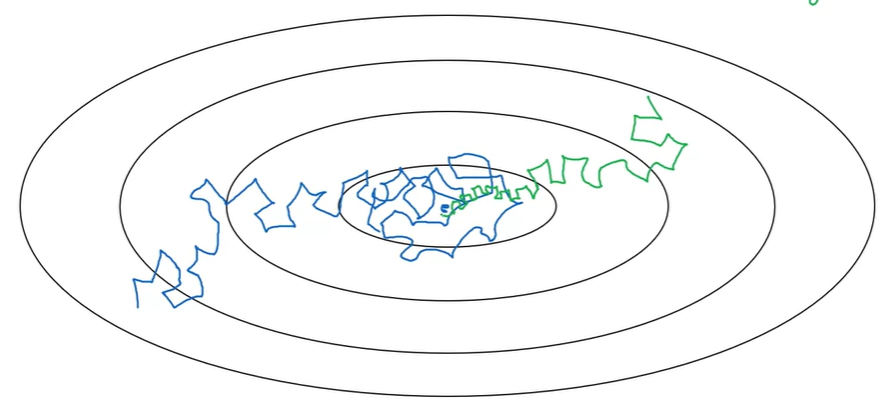
\includegraphics[scale=0.5]{4}\\
				\tabto{0.5cm} Đường màu xanh - learning rate $ \alpha $ cố định\\
				\tabto{0.5cm} Đường màu xanh lá - learning rate $ \alpha $ giảm dần
			\item Công thức:
				\begin{equation*}
				\alpha = \frac{1}{1 + \text{decay-rate} * \text{epoch-num}} \alpha_0
				\end{equation*}
				\begin{itemize}
					\item $ \alpha_0: $ Giá trị learning rate ban đầu
					\item decay-rate: Hyperparameter cần tuning
					\item epoch-num: 1 epoch là 1 lần duyệt qua toàn bộ dữ liệu, epoch-num là số 	lần duyệt qua toàn bộ dữ liệu
				\end{itemize}
			\item Một số công thức khác:
				\begin{itemize}
					\item $ \alpha = 0.95^{\text{epoch-num}} \times \alpha_0 - \text{exponentically decay} $
					\item $ \alpha = \frac{k}{\text{epoch-num}}\alpha_0 $ or $ \frac{k}{\sqrt{t}}\alpha_0 $
					\item Discrete Staircase:\\
						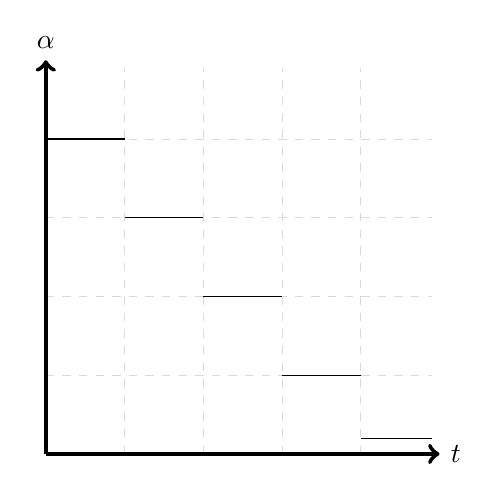
\begin{tikzpicture}
							\draw[help lines, color=gray!30, dashed] (0,0) grid (4.9,4.9);
							\draw[->,ultra thick] (0,0)--(5,0) node[right]{$t$};
							\draw[->,ultra thick] (0,0)--(0,5) node[above]{$\alpha$};
							\draw(0,4)--(1,4);
							\draw(1,3)--(2,3);
							\draw(2,2)--(3,2);
							\draw(3,1)--(4,1);
							\draw(4,0.2)--(4.9,0.2);
						\end{tikzpicture}
					\item Manual Decay: vừa train vừa tự giảm learning rate bằng "cơm"
				\end{itemize}
		\end{itemize}
	\section{The Problem of Local Optima}
		Chỉ cần biết nhớ là: 
		\begin{itemize}
			\item Gần như không thể kẹt ở \textbf{Bad local optima}
			\item \textbf{Plateaus} làm chậm learning \\
				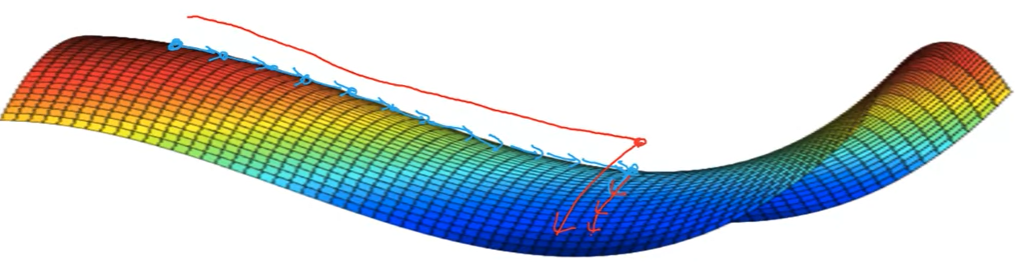
\includegraphics[scale=0.5]{5}
		\end{itemize}
\chapter{Hyperparameter Tuning, Batch Normalization and Programming Frameworks}
	\section{Hyperparameter Tuning}
		\subsection{Tuning Process}
			\begin{itemize}
				\item Ý tưởng: để chọn các giá trị phù hợp của Hyperparameter, ta vẽ theo cặp điểm (ví dụ: $ (\alpha, \epsilon) $) lên trục toạ độ (nhiều chiều hơn thì chỉ 
					xử lý theo phương pháp đại số)
				\item Ví dụ: \\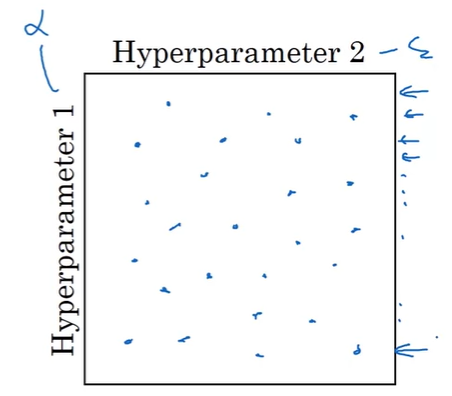
\includegraphics[scale=0.5]{6}\\
					\textbf{Lưu ý:} các điểm được khởi tạo ngẫu nhiên vì: 
					Độ quan trọng của Hyperparameter. \\
					\textit{Tức là hyperparameter $\alpha$ quan trọng hơn $\epsilon$ hay các giá trị $\epsilon$ khác nhau không ảnh hưởng đến thuật toán như $\alpha$ thì 
					nếu như xét ví dụ bên dưới (khởi tạo theo grids) sẽ thử được rất ít giá trị của $\alpha$ so với khởi tạo ngẫu nhiên.}\\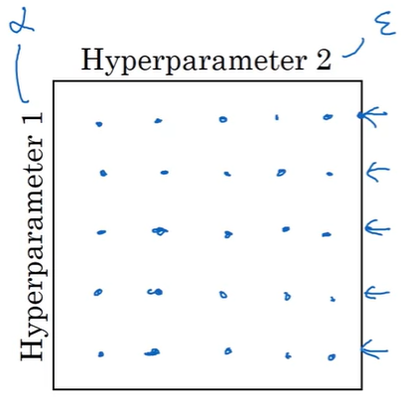
\includegraphics[scale=0.5]{7}
				\item Coarse to fine: Zoom in vào khu vực có các điểm hoạt hoạt động tốt, rồi lại khởi tạo thêm các giá trị \textbf{ngẫu nhiên}, rồi lại chạy 
					thử.\\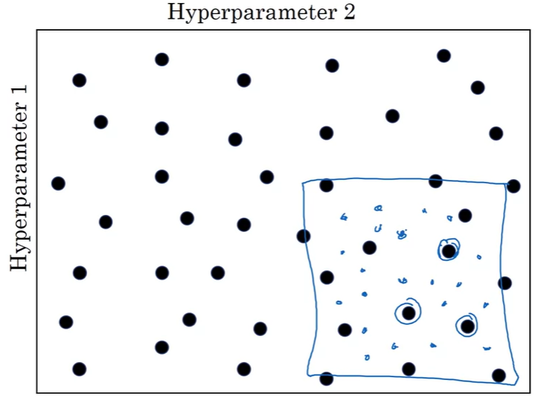
\includegraphics[scale=0.5]{8}
			\end{itemize}
		\subsection{Using an Appropriate Scale to pick Hyperparameters}
			\begin{itemize}
				\item Ý tưởng: chọn khoảng cho Hyperparameter rồi khởi tạo ngẫu nhiên trong khoảng đó
				\item Nếu như cứ dải đều trên khoảng được chọn thì rất cả thể 1 khoảng nào đó sẽ có ít giá trị hơn các khoảng còn lại.\\
					Để khoắc phục thì trên khoảng được chọn, chia nhỏ hơn nữa (theo hàm số mũ $ 10^{-1}, 10^{-2}, ... $), rồi lấy các giá trị ngẫu nhiên trên các khoảng đó
			\end{itemize}
		\subsection{Hyperparameters Tuning in Practice: Pandas vs. Caviar}
			\begin{itemize}
				\item Pandas: train 1 model, mỗi ngày thay đổi hyperparameter 1 tí (phù hợp với dữ liệu lớn, ít phần cứng)
				\item Caviar: train nhiều model cùng lúc với các hyperparameter giống nhau (phù hợp với nhiều phần cứng)
			\end{itemize}
	\section{Batch Normalization}
		\subsection{Normalizing Activations in a Network}
			\begin{itemize}
				\item Ý tưởng: không chỉ normalize Input mà còn normalize cả 
				input $Z$ ở các layer để tính $\omega, b $ tương ứng nhanh hơn
				\item Với một giá trị $ z^{[l](i)} $ bất kì trong Network:\\
				\begin{gather*}
					\mu = \frac{1}{m} \sum_{i} z^{(i)} \\
					\sigma^2 = \frac{1}{m} \sum_{i} (z^{(i)} - \mu)^2 \\
					z^{(i)}_{\text{norm}} = \frac{z^{(i)} - \mu}{\sqrt{\sigma ^2 + \epsilon}} \\
					\tilde{z}^{(i)} = \gamma z^{(i)}_{\text{norm}} + \beta
				\end{gather*}
				\begin{itemize}
					\item $ \gamma, \beta $ là learnable parameters của model
					\item Nếu $ \gamma = \sqrt{\sigma ^2 + \epsilon} $ và $ \beta = \mu $ thì $ \tilde{z}^{(i)} = z^{(i)} $
				\end{itemize}
			\end{itemize}
		\subsection{Fitting Batch Norm into Neural Network}
			\begin{itemize}
				\item Thêm Batch Norm và Network
					\begin{equation*}
						X \xrightarrow{\omega^{[1]}, b^{[1]}} z^{[1]} \xrightarrow[\text{Batch Norm (BN)}]{\beta^{[1]}, \gamma^{[1]}} \tilde{z}^{[1]} \xrightarrow{} a^{[1]} = g^{[1]}(\tilde{z}^{[1]}) \xrightarrow{\omega^{[2]}, b^{[2]}} z^{[2]} \xrightarrow[\text{BN}]{\beta^{[2]}, \gamma^{[2]}} \tilde{z}^{[2]} \xrightarrow{} a^{[2]} \xrightarrow{} \ldots 
					\end{equation*}
				\item Xử lý với Mini-batches
					\begin{equation*}
						X^{\{1\}} \xrightarrow{\omega^{[1]}, b^{[1]}} z^{[1]} \xrightarrow[\text{BN}]{\beta^{[1]}, \gamma^{[1]}} \tilde{z}^{[1]} \xrightarrow{} a^{[1]} = g^{[1]}(\tilde{z}^{[1]}) \xrightarrow{\omega^{[2]}, b^{[2]}} z^{[2]} \xrightarrow[\text{BN}]{\beta^{[2]}, \gamma^{[2]}} \tilde{z}^{[2]} \xrightarrow{} a^{[2]} \xrightarrow{} \ldots 
					\end{equation*}
					\begin{equation*}
						X^{\{2\}} \xrightarrow{\omega^{[1]}, b^{[1]}} z^{[1]} \xrightarrow[\text{BN}]{\beta^{[1]}, \gamma^{[1]}} \tilde{z}^{[1]} \xrightarrow{} a^{[1]} = g^{[1]}(\tilde{z}^{[1]}) \ldots 
					\end{equation*}
					\begin{equation*}
						X^{\{3\}} \xrightarrow{} \ldots
					\end{equation*}
				\item Khi áp dụng Batch Norm thì hyperparameter $ b $ sẽ bị triệt tiêu nên có thể bỏ luôn từ đầu
				\item Implementing Gradient Descent\\
					\tabto{0.5cm} for $ t = 1 \ldots \text{numMiniBatches}  $\\
					\tabto{1cm} Compute forward pop on $ X^{\{t\}} $\\
					\tabto{1.5cm} In each hidden layrer, use BN to replace $ z^{[l]}$ with $\tilde{z}^{[l]}$\\
					\tabto{1cm} Use backpop to compute $ d\omega^{[l]}, d\beta^{[l]}, d\gamma^{[l]} $ (đã bỏ qua $b$)
					\tabto{1cm} Update parameters: $ \omega^{[l]} = \omega^{[l]} - \alpha d\omega^{[l]} $ (tương tự với $ \beta^{[l]}, \gamma^{[l]} $)
					\tabto{0.5cm} Hoạt động với cả Moment, RMSprop, Adam
			\end{itemize}
		\subsection{Why does Batch Norm work?}
			\begin{itemize}
				\item Covariate Shift: vấn đề xảy ra khi phân bố của train set 
				và test set có sự phân bố không đều \textit{(một cách đáng kể)}
				\item Ảnh hưởng của Covariate Shift lên Neural Network:
					\begin{itemize}
						\item Không chỉ trên train set và test set, giữa 2 
						layer của Neural Network cũng xảy ra hiện tượng này.
						\item Vì sự biến đối liên tục của hyperparameter $ 
						\omega, b $ của những layer trước, khiến đầu vào của 
						layer sau chịu ảnh hưởng của Convariate Shift
						\item Batch Norm khiến sự thay đổi đó tác động ít hơn, 
						giúp các layer sau có thể học một cách ổn định hơn vì 
						đầu vào ổn định hơn.
					\end{itemize}
				\item Batch Norm as regularization
					\begin{itemize}
						\item Batch Norm có một chút khả năng regularization, 
						nhưng không đáng kể.
						\item Không thể dựa vào Batch Norm để regularization 
						như Dropout
						\item Giống như Dropout, Batch Norm khiến cho $ z^{[l]} 
						$ hơi bị "noisy" trong Mini-batch, khiến cho layer sau 
						không thể phụ thuộc hoàn toàn vào unit nào của layer 
						trước cả. 	
						\textbf{Tuy nhiên vẫn không có ảnh hưởng như Dropout}
					\end{itemize}										
			\end{itemize}
		\subsection{Batch Norm at Test Time}
			\begin{itemize}
				\item Với test set, chúng ta muốn chạy thử với từng example một 
				chứ không phải là chạy trên từng mini-batch nên không thể dùng 	
				các công thức ở mục 3.2.1 để tính toán $ \mu, \sigma^2 $ rồi 
				đem đi normalize các input.
				\item Để khắc phục vấn đề này thì khi train Neural Network với 
				mini-batch, ta keep track các giá trị $ \mu, \sigma^2 $ rồi áp 
				dụng exponential weight lên chúng để sau khi train model, ta 
				lưu được 1 cặp giá trị $ \mu $ và $ \sigma^2 $, rồi đem cặp giá 
				đó đi normalize input ở test set.
			\end{itemize}
	\section{Multi-class Classification}
			\subsection{Multi-class Classification} 
				\begin{itemize}
					\item Khác bài toàn Logistic ở chỗ: \textbf{Phân biệt nhiều hơn 2 class}
					\item Cách làm thông thường:
						\begin{itemize}
							\item Ở layer cuối của Neural Network sẽ là 1 vecto $ (C, 1) $ ($ C $ là số class cần phân biệt)
							\item Với mỗi phần tử tương ứng với xác suất "Là class đó", phân loại dự trên xác suất cao nhất
							\item Ví dụ: Ta có 3 class cần phân biệt: Méo, Cho, Chim, Khác.\\
								Gán tương ứng: 1, 2, 3, 0\\
								Thì mỗi phần tử của layer cuối sẽ tương ứng: $ P(0|x), P(1|x), P(2|x), P(3|x) $
						\end{itemize}
				\end{itemize}
			\subsection{Softmax Regression} 
				\begin{itemize}
					\item Là thuật toán dùng trong Multi-class Classification
					\item Ý tưởng: activation của layer $ L $ sẽ trả về 1 vecto $ (C, 1) $
					\item Ở layer $ L $:
						\begin{itemize}
							\item $ z^{[L]} = \omega^{[L]} a^{[L-1]} + b^{[L]} $
							\item Activation Function:
								\begin{itemize}
									\item $ t = e^{(z^{[L]})} $
									\item $ a^{[L]} = \frac{e^{(z^{[L]})}}{\sum_{i=1}^4 t_i}( a^{[L]}_i = \frac{t_i}{\sum_{i=1}^4 t_i} )$
								\end{itemize}
						\end{itemize}
				\end{itemize}
			\subsection{Train a Softmax Classifier}
				\begin{itemize}
					\item Softmax Regression generalizes Logistic Regression to 
					$ C $ classes
					\item Loss function:
						\begin{itemize}
							\item $ y = 
								\begin{bmatrix}
									0\\ 1\\ 0\\ 0\\
								\end{bmatrix} $ \qquad
								$ a^{[L]} = \hat{y} = \begin{bmatrix}
									0.3\\ 0.2\\ 0.1\\ 0.4\\
								\end{bmatrix} $
							\item $ \mathcal{L}(\hat{y}, y) = - \displaystyle\sum_{j=1}^{4} y_j \log \hat{y}_j $
							\item $ J(\omega^{[i]}, b^{[i]},...) = \frac{1}{m} \displaystyle\sum_{i=1}^{m} \mathcal{L} (\hat{y}^{(i)}, y^{(i)}) $
							\item $ Y = 
							\begin{bmatrix}
								y^{(1)} & y^{(2)} & ... & y^{(m)}
							\end{bmatrix} = 
							\begin{bmatrix}
								0 & 0 & 1 \\
								1 & 0 & 0 & ...\\
								0 & 1 & 0 \\
								0 & 0 & 0
							\end{bmatrix} (4, m)$ \\
							$ \hat{Y} = 
							\begin{bmatrix}
								\hat{y}^{(1)} & \hat{y}^{(2)} & ... & \hat{y}^{(m)}
							\end{bmatrix} = 
							\begin{bmatrix}
								0.3  \\
								0.2 & ...\\
								0.1 \\
								0.4 
							\end{bmatrix} (4, m)$
						\end{itemize}
				\end{itemize}
\end{document}
